%%%%%%%%%%%%%%%%%%%%%%%%%%%%%%%%%%%%%%%%%
%% Appendix section
% Set-up the section.
%\newpage
\onehalfspacing
\appendix
\setcounter{table}{0}
\renewcommand{\thetable}{A\arabic{table}}
\setcounter{figure}{0}
\renewcommand{\thefigure}{A\arabic{figure}}

% Start appendix
\section{Supplementary Appendix}
\label{appendix}
This section is for supplementary information, and validation of presented propositions and theorems.
It is not meant for publication.

% This project used computational tools which are fully open-source.
%As such, all code and data involved in this project are available at this project's Github repository, available at \url{https://github.com/shoganhennessy/state-faculty-composition}.
%They may be used for replication, or as the basis for further work, as needed.
Any comments or suggestions may be sent to me at \href{mailto:seh325@cornell.edu}{\nolinkurl{seh325@cornell.edu}},
or raised as an issue on the Github project,
\url{https://github.com/shoganhennessy/mediation-natural-experiment}.

\subsection{Identification in Causal Mediation}
\label{appendix:identification}
\citet[Theorem~1]{imai2010identification} states that the ADE and AIE are identified under sequential ignorability, at each level of $Z_i = 0,1$.
For $z' = 0,1$: \\
\makebox[\textwidth]{\parbox{1.25\textwidth}{
\begin{align*}
    \E{ Y_i(1, D_i(z')) - Y_i(0, D_i(z'))}
    &= \int \int 
    \Big( \Egiven{ Y_i }{Z_i = 1, D_i, \vec X_i}
        - \Egiven{ Y_i }{Z_i = 0, D_i, \vec X_i} \Big)
            dF_{D_i \, | \, Z_i = z', \vec X_i} dF_{\vec X_i}, \\
    \E{ Y_i(z', D_i(1)) - Y_i(z', D_i(0))}
    &= \int \int \Egiven{ Y_i }{Z_i = z', D_i, \vec X_i}
    \Big( dF_{D_i \, | \, Z_i = 1, \vec X_i}
        - dF_{D_i \, | \, Z_i = 0, \vec X_i} \Big) dF_{\vec X_i}.
\end{align*}
}}
I focus on the averages, which are identified by consequence of the above.
\begin{align*}
    \E{ Y_i(1, D_i(Z_i)) - Y_i(0, D_i(Z_i))}
    &= \E[Z_i]{\Egiven{ Y_i(1, D_i(z')) - Y_i(0, D_i(z'))}{Z_i = z'}} \\
    \E{ Y_i(Z_i, D_i(1)) - Y_i(Z_i, D_i(0))}
    & = \E[Z_i]{\Egiven{ Y_i(z', D_i(1)) - Y_i(z', D_i(0))}{Z_i = z'}}
\end{align*}
My estimand for the ADE is a simple rearrangement of the above.
The estimand for the AIE relies on a different sequence, relying on (1) sequential ignorability, (2) conditional monotonicity.
These give (1) identification equivalence of AIE local to cpmpliers conditional on $\vec X_i$ and AIE conditional on $\vec X_i$, LAIE $=$ AIE, (2) identification of the complier score.
%, $\Probgiven{D_i(0) = 0, D_i(1) = 1}{\vec X_i}$ $= \Egiven{Y_i}{Z_i, D_i = 1, \vec X_i}
%- \Egiven{Y_i}{Z_i, D_i = 0, \vec X_i}$.
\begin{align*}
    & \Egiven{ Y_i(Z_i, D_i(1)) - Y_i(Z_i, D_i(0))}{\vec X_i} \\
    & = \Probgiven{D_i(0) = 0, D_i(1) = 1}{\vec X_i}
        \Egiven{ Y_i(Z_i, 1) - Y_i(Z_i, 0)}{D_i(0) = 0, D_i(1) = 1, \vec X_i} \\
    & = \Probgiven{D_i(0) = 0, D_i(1) = 1}{\vec X_i}
        \Egiven{ Y_i(Z_i, 1) - Y_i(Z_i, 0)}{\vec X_i} \\
    & = \Probgiven{D_i(0) = 0, D_i(1) = 1}{\vec X_i}
        \; \Big( \Egiven{Y_i}{Z_i, D_i = 1, \vec X_i}
            - \Egiven{Y_i}{Z_i, D_i = 0, \vec X_i} \Big) \\
    & = \Big( \Egiven{D_i}{Z_i = 1, \vec X_i} - \Egiven{D_i}{Z_i = 0, \vec X_i}
        \Big) \;
        \Big( \Egiven{Y_i}{Z_i, D_i = 1, \vec X_i}
            - \Egiven{Y_i}{Z_i, D_i = 0, \vec X_i} \Big)
\end{align*}
Monotonicity is not technically required for the above.
Breaking monotonicity would not change the identification in any of the above; it would be the same except replacing the complier score with a complier/defier score, $\Probgiven{D_i(0) \neq D_i(1)}{\vec X_i} = \Egiven{D_i}{Z_i = 1, \vec X_i} - \Egiven{D_i}{Z_i = 0, \vec X_i}$.

%\subsection{Continuous Average Causal Responses}
%\label{appendix:continuous}
%Section here relating the approach to the average causal response function (see e.g., Angrist Imbens JASA 1996, Andrew Bacon for DiD 2023).

% \subsection{Previous Literature}
% \label{appendix:mediation-review}
% 
% Create a table in this section that surveys previous research which employs mediation methods while having a clear causal design for $Z_i$, but not $D_i$.
%
%\begin{tabular}{l l l l l}
%    Paper & Field & Research Design for $Z_i$ & Research Design for $D_i$ & Selection bias? \\ \hline
%    Paper name 1.    
%\end{tabular}

\subsection{Bias in Causal Mediation (CM) Estimands}
\label{appendix:mediation-bias}
Suppose that $Z_i$ is ignorable conditional on $\vec X_i$, but $D_i$ is not.

\subsubsection{Bias in the Average Direct Effect (ADE)}
To show that the conventional approach to mediation gives an estimate for the ADE with selection and group difference-bias, start with the components of the conventional estimands.
This proof starts with the relevant expectations, conditional on a specific value of $\vec X_i$ and $d' \in \{0, 1 \}$.
\begin{align*}
    \Egiven{Y_i}{Z_i = 1, D_i = d', \vec X_i}
    =& \Egiven{Y_i(1, D_i(Z_i))}{D_i(1) = d', \vec X_i}, \\
    \Egiven{Y_i}{Z_i = 0, D_i = d', \vec X_i}
    =& \Egiven{Y_i(0, D_i(Z_i))}{D_i(0) = d', \vec X_i}
\end{align*}
And so,
\begin{align*}
    &  \Egiven{Y_i}{Z_i = 1, D_i = d', \vec X_i}
    - \Egiven{Y_i}{Z_i = 0, D_i = d', \vec X_i} \\
    &= \Egiven{Y_i(1, D_i(Z_i))}{D_i(1) = d', \vec X_i}
    - \Egiven{Y_i(0, D_i(Z_i))}{D_i(0) = d', \vec X_i} \\
    &= \Egiven{Y_i(1, D_i(Z_i)) - Y_i(0, D_i(Z_i))}{D_i(1) = d', \vec X_i} \\
    &\;\;\;\;+ \Egiven{Y_i(0, D_i(Z_i))}{D_i(1) = d', \vec X_i}
        - \Egiven{Y_i(0, D_i(Z_i))}{D_i(0) = d', \vec X_i}.
\end{align*}
The final term is a sum of the ADE, conditional on $D_i(1) = d'$, and a selection bias term --- difference in baseline outcomes between the (partially overlapping) groups for whom $D_i(1) = d'$ and $D_i(0) = d'$.

To reach the final term, note the following.
\begin{align*}
    &\Egiven{Y_i(1, D_i(Z_i)) - Y_i(0, D_i(Z_i))}{\vec X_i} \\    
    &= \Egiven{Y_i(1, D_i(Z_i)) - Y_i(0, D_i(Z_i))}{D_i(1) = d', \vec X_i} \\
    &\;\;\;\;+ \Big(1 - \Probgiven{D_i(1) = d'}{\vec X_i}\Big)
    \left( \begin{aligned}
        &\Egiven{Y_i(1, D_i(Z_i)) - Y_i(0, D_i(Z_i))}{D_i(1) = d', \vec X_i} \\ 
        & - \Egiven{Y_i(1, D_i(Z_i)) - Y_i(0, D_i(Z_i))}{D_i(1) = 1 - d', \vec X_i}
    \end{aligned} \right) 
\end{align*}
The second term is the difference between the ADE and LADE local to relevant complier groups.

Collect everything together, as follows.
\begin{align*}
    &  \Egiven{Y_i}{Z_i = 1, D_i = d', \vec X_i}
    - \Egiven{Y_i}{Z_i = 0, D_i = d', \vec X_i} \\
    =& \underbrace{
        \Egiven{Y_i(1, D_i(Z_i)) - Y_i(0, D_i(Z_i))}{\vec X_i}}_{
            \text{ADE, conditional on }\vec X_i} \\
    &+ \underbrace{
        \Egiven{Y_i(0, D_i(Z_i))}{D_i(1) = d', \vec X_i}
            - \Egiven{Y_i(0, D_i(Z_i))}{D_i(0) = d', \vec X_i}}_{
                \text{Selection bias}} \\
    &+ \underbrace{\Big(1 - \Probgiven{D_i(1) = d'}{\vec X_i}\Big)
    \left( \begin{aligned}
        &\Egiven{Y_i(1, D_i(Z_i)) - Y_i(0, D_i(Z_i))}{D_i(1) = 1 - d', \vec X_i} \\ 
        & - \Egiven{Y_i(1, D_i(Z_i)) - Y_i(0, D_i(Z_i))}{D_i(1) = d', \vec X_i}
    \end{aligned} \right)}_{
        \text{group difference-bias}}
\end{align*}
The proof is achieved by applying the expectation across $D_i = d'$, and $\vec X_i$.

\subsubsection{Bias in the Average Indirect Effect (AIE)}
To show that the conventional approach to mediation gives an estimate for the AIE with selection and group difference-bias, start with the definition of the ADE --- the direct effect among compliers times the size of the complier group.

This proof starts with the relevant expectations, conditional on a specific value of $\vec X_i$.
\begin{align*}
    &\Egiven{ Y_i(Z_i, D_i(1)) - Y_i(Z_i, D_i(0))}{\vec X_i} \\
    =& \Probgiven{D_i(0) = 0, D_i(1) = 1}{\vec X_i}
        \Egiven{ Y_i(Z_i, 1) - Y_i(Z_i, 0)}{D_i(0) = 0, D_i(1) = 1, \vec X_i}
\end{align*}
When $D_i$ is not ignorable, the bias comes from estimating the second term,
\\ $\Egiven{ Y_i(Z_i, 1) - Y_i(Z_i, 0)}{D_i(0) = 0, D_i(1) = 1, \vec X_i}$, the direct effect among mediator compliers.

Let $z' \in \{ 0, 1 \}$.
Again, note the mean outcomes in terms of average potential outcomes,
\begin{align*}
    \Egiven{Y_i}{Z_i = z', D_i = 1, \vec X_i}
    =& \Egiven{Y_i(z', 1)}{D_i = 1, \vec X_i}, \\
    \Egiven{Y_i}{Z_i = z', D_i = 0, \vec X_i}
    =& \Egiven{Y_i(z', 0)}{D_i = 0, \vec X_i}.
\end{align*}
So compose the selection bias term, as follows.
\begin{align*}
    & \Egiven{Y_i}{Z_i = z', D_i = 1, \vec X_i}
    - \Egiven{Y_i}{Z_i = z', D_i = 0, \vec X_i} \\
    =& \Egiven{Y_i(z', 1)}{D_i = 1, \vec X_i}
        - \Egiven{Y_i(z', 0)}{D_i = 0, \vec X_i} \\
    =& \Egiven{Y_i(z', 1) - Y_i(z', 0)}{D_i = 1, \vec X_i}
    + \Egiven{Y_i(z', 0)}{D_i = 1, \vec X_i} - \Egiven{Y_i(z', 0)}{D_i = 0, \vec X_i}
\end{align*}
The final term is a sum of the AIE, among the treated group $D_i = 1$, and a selection bias term --- difference in baseline potential outcomes between the groups for whom $D_i = 1$ and $D_i = 0$.

The AIE is the direct effect among compliers times the size of the complier group, so we need to compensate for the difference between the treated group $D_i = 1$ and complier group $D_i(0) = 0, D_i(1) = 1$.

Start with the difference between treated group's average and overall average.
\begin{align*}
    & \Egiven{Y_i(z', 1) - Y_i(z', 0)}{D_i = 1, \vec X_i} \\
    =& \Egiven{Y_i(z', 1) - Y_i(z', 0)}{\vec X_i} \\
    &+ \Big(1 - \Probgiven{D_i = 1}{\vec X_i} \Big)
    \left( \begin{aligned}
        &\Egiven{Y_i(z', 1) - Y_i(z', 0)}{D_i = 1, \vec X_i} \\ 
        &  - \Egiven{Y_i(z', 1) - Y_i(z', 0)}{D_i = 0, \vec X_i}
    \end{aligned} \right)
\end{align*}
Then the difference between the compliers' average and the overall average.
\begin{align*}
    & \Egiven{ Y_i(z', 1) - Y_i(z', 0)}{D_i(0) = 0, D_i(1) = 1, \vec X_i} \\
    =& \Egiven{Y_i(z', 1) - Y_i(z', 0)}{\vec X_i} \\
    & + \frac{1 - \Probgiven{D_i(0) = 0, D_i(1) = 1}{\vec X_i} }{
        \Probgiven{D_i(0) = 0, D_i(1) = 1}{\vec X_i}}
    \left( \begin{aligned}
        &\Egiven{Y_i(z', 1) - Y_i(z', 0)}{D_i(1) = 0 \text{ or } D_i(0)=1, \vec X_i} \\ 
        &  - \Egiven{Y_i(z', 1) - Y_i(z', 0)}{\vec X_i}
    \end{aligned} \right)
\end{align*}

Collect everything together, as follows.
\begin{align*}
    &  \Egiven{Y_i}{Z_i = z', D_i = 1, \vec X_i}
    - \Egiven{Y_i}{Z_i = z', D_i = 0, \vec X_i} \\
    =& \underbrace{
        \Egiven{Y_i(z', 1) - Y_i(z', 0)}{D_i(1) =1, D_i(0)=0,\vec X_i}}_{
            \text{AIE among compliers, conditional on }\vec X_i, Z_i = z'} \\
    &+ \underbrace{
        \Egiven{Y_i(z', 0)}{D_i = 1, \vec X_i}
            - \Egiven{Y_i(z', 0)}{D_i = 0, \vec X_i}}_{
                \text{Selection bias}} \\
    &+ \underbrace{\left[ \begin{aligned}
        &\Big( 1 - \Probgiven{D_i = 1}{\vec X_i} \Big)
        \left( \begin{aligned}
            &\Egiven{Y_i(z', 1) - Y_i(z', 0)}{D_i = 1, \vec X_i} \\ 
            &  - \Egiven{Y_i(z', 1) - Y_i(z', 0)}{D_i = 0, \vec X_i}
        \end{aligned} \right) \\
        &- \frac{1 - \Probgiven{D_i(0) = 0, D_i(1) = 1}{\vec X_i} }{
            \Probgiven{D_i(0) = 0, D_i(1) = 1}{\vec X_i}} 
        \left( \begin{aligned}
            &\Egiven{Y_i(z', 1) - Y_i(z', 0)}{D_i(1) = 0 \text{ or } D_i(0)=1, \vec X_i} \\ 
            &  - \Egiven{Y_i(z', 1) - Y_i(z', 0)}{\vec X_i}
        \end{aligned} \right)
    \end{aligned} \right] }_{
        \text{group difference-bias}}
\end{align*}
The proof is finally achieved by multiplying by the complier score, 
$\Probgiven{D_i(0) = 0, D_i(1) = 1}{\vec X_i}$
$= \Egiven{D_i}{Z_i = 1, \vec X_i} - \Egiven{D_i}{Z_i = 0, \vec X_i}$,
then applying the expectation across $Z_i = z'$, and $\vec X_i$.

\subsection{A Regression Framework for Direct and Indirect Effects}
\label{appendix:regression-model}
Put $\mu_{d'}(z'; \vec X) = \Egiven{Y_i(z', d')}{\vec X}$ and $U_{d', i} = Y_i(z', d') - \mu_{d'}(z'; \vec X)$ for each $z',d'=0,1$, so we have the following expressions:
\[ Y_i(Z_i, 0)
        = \mu_{0}(Z_i; \vec X_i) + U_{0,i}, \;\;
    Y_i(Z_i, 1)
        = \mu_{1}(Z_i; \vec X_i) + U_{1,i}. \]
$U_{0,i}, U_{1,i}$ are error terms with unknown distributions, mean independent of $Z_i, \vec X_i$ by definition --- but possibly correlated with $D_i$.
$Z_i$ is conditionally independent of potential outcomes, so that $U_{0,i}, U_{1,i} \indep Z_i$.

The first-stage regression of $Z \to Y$ has unbiased estimates, since $Z_i \indep D_i(.) \big| \vec X_i$.
Put $\pi(z'; \vec X) = \Egiven{D_i(z')}{\vec X}$, and $\eta_{z', i} = D_i(z') - \pi(z'; \vec X)$ the first-stage error terms.
\begin{align*}
    D_i &= Z_i D_i(1) + (1 - Z_i) D_i(0) \\
        &= D_i(0) +
            Z_i \left[ D_i(1) - D_i(0) \right] \\
        &= \underbrace{\pi(0; \vec X_i) 
        }_{\text{Intercept, } \coloneqq \phi + \zeta(\vec X_i)} +
            \underbrace{Z_i \big( \pi(1; \vec X_i) - \pi(0; \vec X_i) \big)}_{
                \text{Regressor, } \coloneqq \bar\pi Z_i }
        + \underbrace{(1- Z_i) \eta_{0,i} + Z_i \eta_{1,i}}_{
            \text{Errors, } \coloneqq \eta_i} \\
    \implies \Egiven{D_i}{Z_i, \vec X_i}
        &= \phi + \bar \pi Z_i + \zeta(\vec X_i).
\end{align*}
Since the ignorability assumption gives $\Egiven{Z_i \eta_{z',i}}{\vec X_i} = \Egiven{Z_i}{\vec X_i} \Egiven{\eta_{z',i}}{\vec X_i} = 0$, for each $z' =0,1$.
By the same argument $Z_i$ is also assumed independent of potential outcomes $Y_i(.,.)$, so that $U_{0,i}, U_{1,i} \indep Z_i$.
Thus, the reduced form regression $Z \to Y$ also leads to unbiased estimates for the ATE.

The same cannot be said of the regression that estimates direct and indirect effects, without further assumptions.
\begin{align*}
    Y_i &= Z_i Y_i(1, D_i(1)) + (1 - Z_i) Y_i(0, D_i(0)) \\
        &= Z_i D_i Y_i(1, 1) \\
        & \;\;\;\; + (1 - Z_i) D_i Y_i(0, 1) \\
        & \;\;\;\; + Z_i (1 - D_i) Y_i(1, 0) \\
        & \;\;\;\; + (1 - Z_i) (1 - D_i) Y_i(0, 0) \\
        &= Y_i(0, 0) \\
        & \;\;\;\; + Z_i \left[Y_i(1, 0) - Y_i(0, 0) \right] \\
        & \;\;\;\; + D_i \left[Y_i(0, 1) - Y_i(0, 0) \right] \\
        & \;\;\;\; + Z_i D_i \left[Y_i(1, 1) - Y_i(1, 0)
            - \left( Y_i(0, 1) - Y_i(0, 0) \right)\right]
\end{align*}
And so $Y_i$ can be written as a regression equation in terms of the observed factors and error terms.
\begin{align*}
    Y_i &= \mu_0(0; \vec X_i) \\
        & \;\;\;\; + D_i \left[\mu_1(0; \vec X_i) - \mu_0(0; \vec X_i) \right] \\
        & \;\;\;\; + Z_i \left[\mu_0(1; \vec X_i) - \mu_0(0; \vec X_i) \right] \\
        & \;\;\;\; + Z_i D_i \left[\mu_1(1; \vec X_i) - \mu_0(1; \vec X_i)
            - \left( \mu_1(0; \vec X_i) - \mu_0(0; \vec X_i) \right)\right] \\
        & \;\;\;\; + U_{0,i} + D_i \left( U_{1,i} - U_{0,i} \right) \\
        &=
            \alpha + \beta D_i + \gamma Z_i + \delta Z_i D_i
            + \varphi(\vec X_i)
            + \left( 1 - D_i \right) U_{0,i} + D_i U_{1,i}
\end{align*}
With the following definitions:
\begin{enumerate}[label=\textbf{(\alph*)}]
    \item $\alpha = \E{\mu_0(0; \vec X_i)}$ and $\varphi(\vec X_i) = \mu_0(0; \vec X_i) - \alpha$ are the intercept terms.
    \item $\beta = \mu_1(0; \vec X_i) - \mu_0(0; \vec X_i)$ is the indirect effect under $Z_i = 0$
    \item $\gamma = \mu_0(1; \vec X_i) - \mu_0(0; \vec X_i)$ is the direct effect under $D_i = 0$.
    \item $\delta = \mu_1(1; \vec X_i) - \mu_0(1; \vec X_i)- \left( \mu_1(0; \vec X_i) - \mu_0(0; \vec X_i) \right)$ is the interaction effect.
    \item $\left( 1 - D_i \right) U_{0,i} + D_i U_{1,i}$ is the remaining error term.
\end{enumerate}
This sequence gives us the resulting regression equation:
\begin{align*}
    \Egiven{Y_i}{Z_i, D_i, \vec X_i} \;\; =& \;\;
        \alpha
        + \beta D_i
        + \gamma Z_i
        + \delta Z_i D_i
        + \varphi(\vec X_i) \\
        & \;\; +\left( 1 - D_i \right) \Egiven{ U_{0,i} }{D_i = 0, \vec X_i}
            + D_i \Egiven{ U_{1,i} }{D_i = 1, \vec X_i}
\end{align*}
Taking the conditional expectation, and collecting for the expressions of the direct and indirect effects:
\begin{align*}
    \E{Y_i(1, D_i(Z_i)) - Y_i(0, D_i(Z_i))}
        &= \E{\gamma + \delta D_i} \\
    \E{Y_i(Z_i, D_i(1)) - Y_i(Z_i, D_i(0))}
        &= \E{\bar \pi \left( \beta +  Z_i \delta + \tilde U_i \right)}
\end{align*}
These equations have simpler expressions after assuming constant treatment effects in a linear framework;
I have avoided this as having compliers, and controlling for observed factors $\vec X_i$ only makes sense in the case of heterogeneous treatment effects.

These terms are conventionally estimated in a simultaneous regression \citep{imai2010identification}.
If sequential ignorability does not hold, then the regression estimates from estimating the mediation equations (without adjusting for the contaminated bias term) suffer from omitted variables bias.

\makebox[\textwidth]{\parbox{1.25\textwidth}{
\begin{align*}
    \E[\vec X_i]{\Egiven{Y_i}{Z_i = D_i = 0, \vec X_i}}
        &= \E\alpha + \Egiven{ U_{0,i} }{D_i = 0} \\
    \E[\vec X_i]{\Egiven{Y_i}{Z_i = 0, D_i = 1, \vec X_i}
        - \Egiven{Y_i}{Z_i = 0, D_i = 0, \vec X_i}}
        &= \E\beta + 
            \left( \Egiven{ U_{1,i} }{D_i = 1} - \Egiven{ U_{0,i} }{D_i = 0} \right) \\
    \E[\vec X_i]{\Egiven{Y_i}{Z_i = 1, D_i = 0, \vec X_i}
        - \Egiven{Y_i}{Z_i = 0, D_i = 0, \vec X_i}}
        &= \E\gamma + \Egiven{ U_{0,i} }{D_i = 0} \\
    \E[\vec X_i]{\begin{aligned}
        &\Egiven{Y_i}{Z_i = 1, D_i = 1, \vec X_i}
            - \Egiven{Y_i}{Z_i = 1, D_i = 0, \vec X_i} \\
            &- \left( \Egiven{Y_i}{Z_i = 0, D_i = 1, \vec X_i}
                - \Egiven{Y_i}{Z_i = 0, D_i = 0, \vec X_i} \right)
        \end{aligned}}
    &= \E\delta
\end{align*}
}}
And so the ADE and AIE estimates are contaminated by these bias terms.
Additionally, the AIE estimates refers to gains from the mediator among $D(z)$ compliers (not the entire average), so will be biased when not accounting for $\tilde U_i$, too.

\subsection{Roy Model and Sequential Ignorability}
\label{appendix:roy-seq-ig}
\textit{Proof of Proposition \ref{prop:roy-seq-ig}.}

Suppose $Z_i$ is ignorable, and selection-into-$D_i$ follows a Roy model, with the definitions in \autoref{sec:applied}.
If selection-into-$D_i$ is degenerate on $U_{0,i}, U_{1,i}$:
\[ \Egiven{D_i}{Z_i, \vec X_i, U_{1,i}- U_{0,i} = u}
    = \Egiven{D_i}{Z_i, \vec X_i, U_{1,i}- U_{0,i} = u'},
    \text{ for all } u, u' \text{ in the range of $U_{1,i}- U_{0,i}$.} \]
%Conversely, if selection based on $U_{0,i}, U_{1,i}$ is non-degenerate:
%\[ \exists u, u' \text{in the range of $U_{1,i}- U_{0,i}$ such that }
%    \Egiven{D_i}{Z_i, \vec X_i, U_{1,i}- U_{0,i} = u}
%    \neq \Egiven{D_i}{Z_i, \vec X_i, U_{1,i}- U_{0,i} = u'}. \]
    %, \;\;\; \text{for at least one } z'=0,1 \]
In this case, the control set $\vec X_i$ and the costs $\mu_c, U_{c,i}$ are the only determinants of selection-into-$D_i$ --- and, $U_{0,i}, U_{1,i}$ play no role.
This could be achieved by either assuming that unobserved gains are degenerate (the researcher had observed everything in $\vec X_i$), or selection-into-$D_i$ had been disrupted in some fashion (e.g., by a natural experiment design for $D_i$).

To motivate a contraposition argument, suppose $D_i$ is ignorable conditional on $Z_i, \vec X_i$.
For each $z', d' = 0, 1$
\begin{align*}
    & D_i \indep Y_i(z', d') \;\; | \;\; \vec X_i, Z_i = z' \\
    &\implies D_i \indep \mu_{d'}(z'; \vec X_i) + U_{d',i} \;\; | \;\; \vec X_i, Z_i = z' \\
    &\implies D_i \indep U_{d',i} \;\; | \;\; \vec X_i, Z_i = z' \\
    &\implies D_i \indep U_{1,i} - U_{0,i} \;\; | \;\; \vec X_i, Z_i = z' \\
    &\implies \Egiven{D_i}{U_{1,i} - U_{0,i} = u', \vec X_i, Z_i = z'}
    = \Egiven{D_i}{\vec X_i, Z_i = z'} \\
    & \;\;\; \;\;\; \;\;\; \text{for all } u' \text{ in the range of $U_{1,i}- U_{0,i}$.}
\end{align*}
This final implication is that selection-into-$D_i$ is degenerate on $U_{0,i}, U_{1,i}$.
Thus, a contraposition argument has that if selection-into-$D_i$ is non-degenerate on $U_{0,i}, U_{1,i}$, then $D_i$ is not ignorable.

% Consider the following case, for each individual $i$.
% \[ \bar u_i = \mu_C(Z_i ; \vec X_i) + U_{C,i} - \mu(Z_i ; \vec X_i) \]
% $\Egiven{D_i}{U_i = \bar u, \vec X_i, Z_i} = 1$, so that
% The range of $U_{1,i}- U_{0,i}$ must contain at least two entries, one greater(or equal) to $\bar u_i$ (call it $u_i$), and another smaller than $\bar u_i$ (call it $u_i'$) for each $i$.
% \[ 1 = \Egiven{D_i}{U_i = u_i, \vec X_i, Z_i} \neq 
% \Egiven{D_i}{U_i = u_i', \vec X_i, Z_i} = 0 \]
% Now we reach a contradiction, because $u, u'$ were defined in terms of the mean potential outcomes $\mu(z';.)$, and thus conditional mean depends on the potential outcomes.

\subsection{Monotonicity $\implies$ Selection Model, in a CM Setting.}
\label{appendix:cf-monotonicity}
\textit{Proof that (conditional) monotonicity implies a selection model representation in a CM setting.
    This proof is an applied example of the \cite{vytlacil2002independence} equivalence result, now including conditioning covariates $\vec X_i$, and is presented merely as a validation exercise.
}

Assume condition monotonicity \ref{cf:monotonicity} holds, for any treatment values $z < z'$ and any covariate value $\vec X_i = \vec x$.
\[ \Probgiven{D_i(z') \geq D_i(z)}{\vec x} = 1. \]
For each value of $\vec{X}_i = \vec{x}$ and any treatment values $z < z'$, we first define:
\begin{itemize}
    \item $\mathcal{A} = \{i : D_i(z) = D_i(z') = 1\}$, always-mediators
    \item $\mathcal{N} = \{i : D_i(z) = D_i(z') = 0\}$, never-mediators
    \item $\mathcal{C} = \{i : D_i(z) = 0, D_i(z') = 1\}$, mediator-compliers.
\end{itemize}
For any mediator complier $i \in \mathcal C$, partition the set as follows.
\begin{itemize}
    \item $\mathcal{Z}_1(i) = \{z' : D_i(z') = 1\}$, treatment values where $i$ takes the mediator
    \item $\mathcal{Z}_0(i) = \{z' : D_i(z') = 0\}$, treatment values where $i$ doesn't take the mediator.
\end{itemize}
Note that having binary $Z_i = 0,1$ reduces this to the simple case of $\mathcal{Z}_0(i) = \{0\}$, and $\mathcal{Z}_1(i) = \{1\}$.
The equivalence result holds for continuous values of $Z_i$, so continue with the more general $\mathcal{Z}_0(i), \mathcal{Z}_1(i)$ notation.

By monotonicity, we have
\[ \sup_{z' \in \mathcal{Z}_0(i)} \pi(z';\vec{x})
    \leq \inf_{z' \in \mathcal{Z}_1(i)} \pi(z';\vec{x}), \;\;
    \text{ for any } i \in \mathcal{C} \]
where $\pi(z';\vec{x}) = \Probgiven{D_i = 1}{Z_i = z', \vec{X}_i = \vec{x}}$ is the mediator propensity score.
A simple proof by contradiction verifies this statement (\citealt[Lemma 1]{vytlacil2002independence}).

Now we construct $V_i$ as follows:
\[ V_i = 
    \begin{cases}
        1, & \text{if } i \in \mathcal{N} \\
        0, & \text{if } i \in \mathcal{A} \\
        \inf_{z' \in \mathcal{Z}_1(i)} \pi(z';\vec{x}), & \text{if } i \in \mathcal{C}.
    \end{cases} \]
Define $\psi(z';\vec{x}) = \pi(z';\vec{x})$.
Then we can represent $D_i(z')$ as a selection model,
\[ D_i(z') = \indicator{\psi(z';\vec{X}_i) \geq V_i}, \;\text{ for } z'=0,1. \]
We can verify this works:
\begin{itemize}
    \item For $i \in \mathcal{A}$: $V_i = 0$ and $\psi(z';\vec{x}) \geq 0$ for all $z'$, so $D_i(z') = 1$
    
    \item For $i \in \mathcal{N}$: $V_i = 1$ and $\psi(z';\vec{x}) \leq 1$ for all $z'$, with $\psi(z';\vec{x}) < 1$ for $z' \in \mathcal{Z}_0(i)$, so $D_i(z') = 0$ for $z' \in \mathcal{Z}_0(i)$
    
    \item For $i \in \mathcal{C}$: $V_i = \inf_{z' \in \mathcal{Z}_1(i)} \pi(z';\vec{x})$
    \begin{itemize}
        \item When $z' \in \mathcal{Z}_1(i)$: $\psi(z';\vec{x}) \geq \inf_{z'' \in \mathcal{Z}_1(i)} \pi(z'';\vec{x}) = V_i$, so $D_i(z') = 1$
        \item When $z' \in \mathcal{Z}_0(i)$: $\psi(z';\vec{x}) < \inf_{z'' \in \mathcal{Z}_1(i)} \pi(z'';\vec{x}) = V_i$, so $D_i(z') = 0$.
    \end{itemize}
\end{itemize}
Therefore, the construction $D_i(z') = \indicator{\psi(z';\vec{X}_i) \geq V_i}$ is a valid representation of the selection process under monotonicity.

This selection model can be transformed to one with a uniform distribution, to get the general selection model of \cite{heckman2005structural}.
Let $F_V \big( .\, \big|\, \vec{X}_i \big)$ be the conditional cumulative density function of $V_i$ given $\vec{X}_i$.
Define
\begin{align*}
    U_i &= F_V \left( V_i \mid \vec{X}_i \right) \\
    \pi(z'; \vec{X}_i) 
        &= F_V\left( \psi(z'; \vec{X}_i) \mid \vec{X}_i \right)
        = \Probgiven{D_i = 1}{Z_i = z', \vec{X}_i}
\end{align*}
We can then equivalently represent the mediator choice as the transformed selection model
\[ D_i(z') = \indicator{\pi(z'; \vec{X}_i) \geq U_i}, \;\;\; \text{for } z'=0,1 \]
where $U_i \,| \,\vec{X}_i \sim \text{Uniform}(0,1)$ by the probability integral transformation.

\subsection{Control Function (CF) Identification of the Second-stage}
\label{appendix:cf-secondstage}
\textit{Proof of Proposition \ref{proposition:secondstage}.
    This proof relies heavily on the notation and reasoning of \cite{kline2019heckits} for an IV setting.}

By Assumption \ref{cf:monotonicity} (mediator monotonicity), selection-into-mediator can be represented as a threshold-crossing selection model.
\[ D_i(z') = \indicator{ \pi(z'; \vec X_i) \geq U_i }, \text{ for } z' = 0, 1 \]
where $U_i = F_V\left( V_i \mid \vec{X}_i \right)$ follows a uniform distribution on $[0,1]$, and $\pi(z'; \vec X_i) = \Egiven{D_i}{Z_i = z', \vec X_i}$ is the mediator propensity score.

The threshold crossing selection model represents individuals who refuse the mediator as follows:
\[ D_i = 0 \implies \pi(Z_i; \vec X_i) < U_i \]
Our objective is to determine $\Egiven{U_{0,i}}{D_i=0, Z_i, \vec X_i}$, which can then be written as
\[ \Egiven{U_{0,i}}{\pi(Z_i; \vec X_i) < U_i, Z_i, \vec X_i}. \]
Since $Z_i$ is ignorable, we have:
\[ \Egiven{U_{0,i}}{\pi(Z_i; \vec X_i) < U_i, Z_i, \vec X_i}
    = \Egiven{U_{0,i}}{\pi(Z_i; \vec X_i) < U_i} \]

Assumption \ref{cf:identification} has $\text{Cov}(U_i, U_{0,i}) \neq 0$.
This non-zero covariance implies statistical dependence between the selection error and outcome error.
This dependence allows us to represent $U_{0,i}$ using a linear projection.
We use $F_V^{-1}\left( U_i \mid \vec{X}_i \right)$ rather than $U_i$ directly in the projection to allow for flexibility in how the selection error affects outcomes.
The linear projection can be written as follows
\[ U_{0,i} = \rho_0 \big( F_V^{-1}\left( U_i \mid \vec{X}_i \right) - \mu_V \big) + \varepsilon_{0,i}, \]
where
\begin{itemize}
    \item $\mu_V = \E{F_V^{-1}\left( U_i \mid \vec{X}_i \right)}$ is the mean of $F_V^{-1}\left( U_i \mid \vec{X}_i \right)$
    \item $\rho_0 = \frac{\Cov{U_{0,i}, F_V^{-1}\left( U_i \mid \vec{X}_i \right)}}{\Var{F_V^{-1}\left( U_i \mid \vec{X}_i \right)}}$ is the projection coefficient
    \item $\varepsilon_{0,i}$ is a residual with $\Egiven{\varepsilon_{0,i}}{F_V^{-1}\left( U_i \mid \vec{X}_i \right)} = 0$.
\end{itemize}

The coefficient $\rho_0$ is the slope in the best linear predictor of $U_{0,i}$ given $F_V^{-1}\left( U_i \mid \vec{X}_i \right)$, and is chosen to ensure that the residual $\varepsilon_{0,i}$ is uncorrelated with $F_V^{-1}\left( U_i \mid \vec{X}_i \right)$.
This property is crucial for the identification strategy, as it isolates the component of $U_{i}$ that is related to selection-into-$D_i$.

The non-zero covariance condition in \ref{cf:identification} ensures $\rho_0 \neq 0$, so is relevant.
Since $U_i$ and $F_V^{-1}\left( U_i \mid \vec{X}_i \right)$ are related by a monotonic transformation (the inverse cumulative density function), the covariance $\text{Cov}(U_i, U_{0,i}) \neq 0$ implies $\text{Cov}(F_V^{-1}\left( U_i \mid \vec{X}_i \right), U_{0,i}) \neq 0$.

Given the linear projection of $U_{0,i}$ onto $F_V^{-1}\left( U_i \mid \vec{X}_i \right)$, we can compute the conditional expectation:
\[ \Egiven{U_{0,i}}{\pi(Z_i; \vec X_i) < U_i} = \Egiven{\rho_0\big(F_V^{-1}\left( U_i \mid \vec{X}_i \right) - \mu_V\big) + \varepsilon_{0,i}}{\pi(Z_i; \vec X_i) < U_i} \]

Since $\Egiven{\varepsilon_{0,i}}{F_V^{-1}\left( U_i \mid \vec{X}_i \right)} = 0$ by construction, and $U_i$ is a function of $F_V^{-1}\left( U_i \mid \vec{X}_i \right)$, we have
\[ \Egiven{\varepsilon_{0,i}}{\pi(Z_i; \vec X_i) < U_i} = 0. \]

Therefore:
\[ \Egiven{U_{0,i}}{\pi(Z_i; \vec X_i) < U_i} = \rho_0 \Egiven{F_V^{-1}\left( U_i \mid \vec{X}_i \right) - \mu_V}{\pi(Z_i; \vec X_i) < U_i}. \]

This gives us the control function representation:
\[ \Egiven{U_{0,i}}{D_i=0, Z_i, \vec X_i} = \rho_0 \lambda_0\big(\pi(Z_i; \vec X_i)\big) \]
where $\lambda_0 \left(p'\right) = \Egiven{F_V^{-1}\left( U_i \mid \vec{X}_i \right) - \mu_V}{p' < U_i}$.
The control function $\lambda_0\left(p'\right)$ captures the expected value of the transformed selection term, conditional on being above the threshold $p' \in (0,1)$.

The same sequence of steps for mediator takers, $D_i = 1$, gives the other CF:
\[ \Egiven{U_{1,i}}{D_i=1, Z_i, \vec X_i} = \rho_1 \lambda_1\big(\pi(Z_i; \vec X_i)\big), \]
where $\lambda_1 \left(p'\right) = \Egiven{F_V^{-1}\left( U_i \mid \vec{X}_i \right) - \mu_V}{U_i \leq p'}$ for $p' \in (0,1)$, and $\rho_1 = \frac{\Cov{U_{1,i}, F_V^{-1}\left( U_i \mid \vec{X}_i \right)}}{\Var{F_V^{-1}\left( U_i \mid \vec{X}_i \right)}}$ is the corresponding projection coefficient.

The relationship between $\lambda_0(p')$ and $\lambda_1(p')$ can be derived as:
\[ \lambda_1 \left(p'\right) = -\lambda_0 \left(p'\right) \left( \frac{1-p'}{p'} \right), \text{ for } p' \in (0,1). \]
This relationship ensures consistency in the CF approach across the $D_i=0$ and $D_i= 1$ groups \citep{kline2019heckits}.

Assumption \ref{cf:instrument} (mediator take-up cost instrument $\vec X_i^{\text{IV}}$) ensures identification of the propensity score function $\pi(z'; \vec X_i)$ in the first stage by providing valid instrumental variation.
This variation allows us to identify the propensity score, and consequently the control functions $\lambda_0$ and $\lambda_1$.

Combining all elements, the conditional expectation of $Y_i$ given $Z_i, D_i, \vec X_i$ is
\begin{align*}
    \Egiven{Y_i}{Z_i, D_i, \vec X_i} \;\; =& \;\;
        \alpha
        + \beta D_i
        + \gamma Z_i
        + \delta Z_i D_i
        + \varphi(\vec X_i) \\
        & \;\; + \left( 1 - D_i \right) \Egiven{U_{0,i}}{D_i = 0}
            + D_i \Egiven{U_{1,i}}{D_i = 1}.
\end{align*}
Substitute the CFs,
\begin{align*}
    &\;(1-D_i) \Egiven{ U_{0,i} }{Z_i, D_i=0, \vec X_i}
        + D_i \Egiven{ U_{1,i}}{Z_i, D_i=1, \vec X_i} \\
    &=\; (1-D_i)\rho_0 \lambda_0 \big(\pi(Z_i; \vec X_i) \big)
    + D_i \rho_1 \lambda_1 \big(\pi(Z_i; \vec X_i) \big).
\end{align*}
This gives the final result,
\begin{align*}
    \Egiven{Y_i}{Z_i, D_i, \vec X_i} \;\; =& \;\;
        \alpha
        + \beta D_i
        + \gamma Z_i
        + \delta Z_i D_i
        + \varphi(\vec X_i) \\
        & \;\; +  \rho_0 \left( 1 - D_i \right) \lambda_0 \big( \pi(Z_i ; \vec X_i) \big)
            + \rho_1 D_i \lambda_1 \big( \pi(Z_i ; \vec X_i) \big).
\end{align*}
All parameters --- $\alpha, \beta, \gamma, \delta, \varphi(.), \rho_0, \rho_1$ --- are identified once we control for selection bias through the CFs $\lambda_0, \lambda_1$, with $\pi(z';\vec X_i)$ identified separately in the first-stage.
$\lambda_0, \lambda_1$ can be assumed to be certain functions (say, the inverse Mills ratio in \citealt{heckman1979sample}), or treated as non-parametric parameters to be estimated with the moment equality $\lambda_1 \left(p'\right) = -\lambda_0 \left(p'\right) \left( \frac{1-p'}{p'} \right)$ for $p \in (0,1)$.

\subsection{Control Function (CF) Identification of the ADE and AIE}
\label{appendix:cf-ade-aie}
\textit{Proof of Theorem \ref{thm:cf-identification}.}

Assume \ref{cf:monotonicity}, \ref{cf:identification}, \ref{cf:instrument} hold.
Then Proposition~\ref{proposition:secondstage} has $\alpha, \beta, \gamma, \delta, \varphi(.), \rho_0, \rho_1$ identified in a regression.
The following composes the ADE and AIE from these parameters.

For the ADE,
\begin{align*}
    \E{ \gamma + \delta D_i}
        &= \E{ \Big( \mu_0(1; \vec X_i) - \mu_0(0; \vec X_i) \Big)
            + D_i \Big( \mu_1(1; \vec X_i) - \mu_0(1; \vec X_i) - \big( \mu_1(0; \vec X_i) - \mu_0(0; \vec X_i) \big) \Big) } \\
    &= \E{ D_i \Big(\mu_1(1; \vec X_i) - \mu_1(0; \vec X_i) \Big)
        + (1 - D_i) \Big( \mu_0(1; \vec X_i) - \mu_0(0; \vec X_i) \Big) } \\
    &= \E{ D_i \Big( Y_i(1,1) - U_{1,i} - \big( Y_i(0,1) - U_{1,i} \big) \Big)
        + (1 - D_i) \Big( 
            Y_i(1,0) - U_{0,i} - \big( Y_i(0,0) - U_{0,i} \big) \Big) } \\
    &= \E{ D_i \Big( Y_i(1,1) - Y_i(0,1) \Big)
        + (1 - D_i) \Big( Y_i(1,0) - Y_i(0,0) \Big) } \\
    &= \E{ Y_i(1, D_i(Z_i)) - Y_i(0, D_i(Z_i))} \\
    &= \text{ADE}.
\end{align*}

Identification is similar for the AIE, but also involves the complier adjustment term.
\begin{align*}
    (\rho_1 - \rho_0) \, \Gamma \big(\pi(0; \vec{X}_i), \, \pi(1; \vec{X}_i) \big)
    &= (\rho_1 - \rho_0) \, \frac{\pi(1; \vec{X}_i)\lambda_1(\pi(1; \vec{X}_i)) - \pi(0; \vec{X}_i)\lambda_1(\pi(0; \vec{X}_i))}{\pi(1; \vec{X}_i) - \pi(0; \vec{X}_i)} \\
    &= (\rho_1 - \rho_0) \, \Egiven{ F_V^{-1}(U_i | \vec{X}_i) - \mu_V }{\pi(0; \vec{X}_i) < U_i \leq \pi(1; \vec{X}_i), \vec{X}_i} \\
    &= (\rho_1 - \rho_0) \, \Egiven{ F_V^{-1}(U_i | \vec{X}_i) - \mu_V }{
        D_i(0) = 0, D_i(1) = 1, \vec{X}_i} \\
    &= \Egiven{ \rho_1 \big( F_V^{-1}(U_i | \vec{X}_i) - \mu_V \big) }{
        D_i(0) = 0, D_i(1) = 1, \vec{X}_i} \\
    &\;\;\; - \Egiven{ \rho_0 \big( F_V^{-1}(U_i | \vec{X}_i) - \mu_V \big) }{
        D_i(0) = 0, D_i(1) = 1, \vec{X}_i} \\
    &= \Egiven{ U_{1,i} - U_{0,i} }{D_i(0) = 0, D_i(1) = 1, \vec{X}_i}.
\end{align*}
This complier adjustment was first presented for an IV setting by \cite{kline2019heckits}.

Collecting for the AIE,
\begin{align*}
    &\E{ \bar \pi \, \Big( \beta +  \delta Z_i +
        (\rho_1 - \rho_0) \Gamma \big(\pi(0; \vec X_i), \, \pi(1; \vec X_i) \big) \Big) } \\
    &= \E{ \bar \pi \, \Bigg( \Big( \mu_1(0; \vec X_i) - \mu_0(0; \vec X_i) \Big)
        +  Z_i \Big( \mu_1(1; \vec X_i) - \mu_0(1; \vec X_i)
            - \big(\mu_1(0; \vec X_i) - \mu_0(0; \vec X_i) \big) \Big) \Bigg) } \\
    &\;\;\;\; + \mathbb E \Big[ \bar \pi \; \Egiven{ U_{1,i} - U_{0,i} }{D_i(0) = 0, D_i(1) = 1, \vec{X}_i} \Big] \\
    &= \E{ \bar \pi \, \Bigg(
        Z_i \Big( \mu_1(1; \vec X_i) - \mu_0(1; \vec X_i) \Big)
        + (1 - Z_i) \Big( \mu_1(0; \vec X_i) - \mu_0(0; \vec X_i) \Big) \Bigg) } \\
    &\;\;\;\; + \mathbb E \Big[ \bar \pi \; \Egiven{ U_{1,i} - U_{0,i} }{D_i(0) = 0, D_i(1) = 1, \vec{X}_i} \Big] \\
    &= \E{ \bar \pi \, \Bigg(
        \mu_1(Z_i, \vec X_i) - \mu_0(Z_i, \vec X_i)
        + \Egiven{ U_{1,i} - U_{0,i} }{D_i(0) = 0, D_i(1) = 1, \vec{X}_i} \Bigg) } \\
    &= \E{ \bar \pi \; \Egiven{
        \mu_1(Z_i, \vec X_i) - \mu_0(Z_i, \vec X_i) + U_{1,i} - U_{0,i} }{
            D_i(0) = 0, D_i(1) = 1, \vec{X}_i} } \\
    &= \E{ \Egiven{D_i(1) - D_i(0)}{\vec X_i} \; \Egiven{
        Y_i(Z_i, 1) - Y_i(Z_i, 0) }{ D_i(0) = 0, D_i(1) = 1, \vec{X}_i} } \\
    &= \E{ \Egiven{Y_i(Z_i,D_i(1)) - Y_i(Z_i,D_i(0))}{\vec X_i} } \\
    &= \E{ Y_i(Z_i,D_i(1)) - Y_i(Z_i,D_i(0)) } \\
    &= \text{AIE}.
\end{align*}

\subsection{Semiparametric Estimation of the ADE and AIE}
\label{appendix:semiparametric}
Note the following, to express $\Gamma(p,p')$ in terms of either $\lambda_0$ or $\lambda_1$
for $p < p' \in (0,1)$.
\begin{align*}
    \Gamma\left(p,p'\right) 
        &= \Egiven{ F_V^{-1}\left( U_i \mid \vec{X}_i \right) - \mu_V}{p < U_i \leq p'} \\
        &= \frac{p'\lambda_1\left(p'\right) - p\lambda_1\left(p\right)}{p' - p} \\
        &= \frac{(1-p)\lambda_0\left(p\right) - (1-p')\lambda_0\left(p'\right)}{p' - p} \\
\end{align*}

The semiparametric approach cannot separate $\rho_0$ from $\lambda_0$, only estimating their composition $\rho_0 \lambda_0(p')$ for $p' \in (0,1)$.
Ultimately this does not matter, as it sufficient to identify $\rho_0, \rho_1$ up to a constant for the complier adjustment term, using either $\rho_0 \lambda_0$ or $\rho_1 \lambda_1$.
For $\pi_0 < \pi_1 \in (0,1)$,
\begin{align*}
    (\rho_1 - \rho_0) \, \Gamma \big(\pi_0, \pi_1 \big)
    &= (\rho_1 - \rho_0) \frac{\pi_1\lambda_1\left(\pi_1\right) - \pi_0\lambda_1\left(\pi_0\right)}{\pi_1 - \pi_0} \\
    &= \left(1 - \frac{\rho_0}{\rho_1}\right) \frac{
        \pi_1 \rho_1 \lambda_1\left(\pi_1\right) - \pi_0 \rho_1 \lambda_1\left(p\right)}{\pi_1 - \pi_0} \\
    &= \left(\frac{\rho_1}{\rho_0} - 1 \right) \frac{
        (1 - \pi_0) \rho_0 \lambda_0\left(\pi_0\right) - (1 - \pi_1) \rho_0 \lambda_0\left(\pi_1\right)}{\pi_1 - \pi_0}.
\end{align*}

The fraction $\rho_1 / \rho_0$ can be estimated with only the composition $\rho_0 \lambda_0$ or $\rho_1 \lambda_1$, thanks to the relation between $\lambda_0, \lambda_1$.
For $p' \in (0,1)$,
\[ \lambda_1 \left(p'\right) = 
    \implies 
        \frac{\rho_0}{\rho_1} = 
        \frac{\rho_0 \lambda_0 \left(p'\right)}{ \rho_1 \lambda_1 \left(p'\right)}
        \left( \frac{1-p'}{p'} \right). \]
This can be estimated by estimating $\rho_1 \lambda_1$ in the $D_i = 1$ subsample with splines, extrapolating the transformed $\rho_1 \lambda_0(p') = -\rho_1\lambda_1 \left(p'\right) \left( \frac{p'}{1 - p'} \right)$ to the $D_i = 0$ subsample, and calculating the regression coefficient for $\rho_0 / \rho_1$ on $\rho_1 \lambda_0(p')$.

Similarly, an approach starting with estimating $\rho_0 \lambda_0$ in the $D_i = 0$ subsample gives a coefficient for $\rho_1 / \rho_0$.
An efficient estimate can compose these two, with weights proportional to the efficiency of each side.

\subsection{Control Function Simulation}
A number of statistical packages, for the R language \citep{R2023}, made the simulation analysis for this paper possible.
\begin{itemize}
    \item \textit{Tidyverse} \citep{tidyverse} collected tools for data analysis in the R language.
    \item \textit{Splines} \citep{wang2021shape} allows semi-parametric estimation, using splines, in the R language.
    \item \textit{Mediate} \citep{tingley2014mediation} automates the sequential-ignorability estimates of CM effects \citep{imai2010identification} in the R language.
\end{itemize}

\begin{figure}[h!]
    \caption{Point Estimates of CM Effects, OLS and Control Function versus True Value.}
    \begin{subfigure}[c]{0.475\textwidth}
        \centering
        \caption{$\hat{\text{ADE}} \;-$ ADE.}
        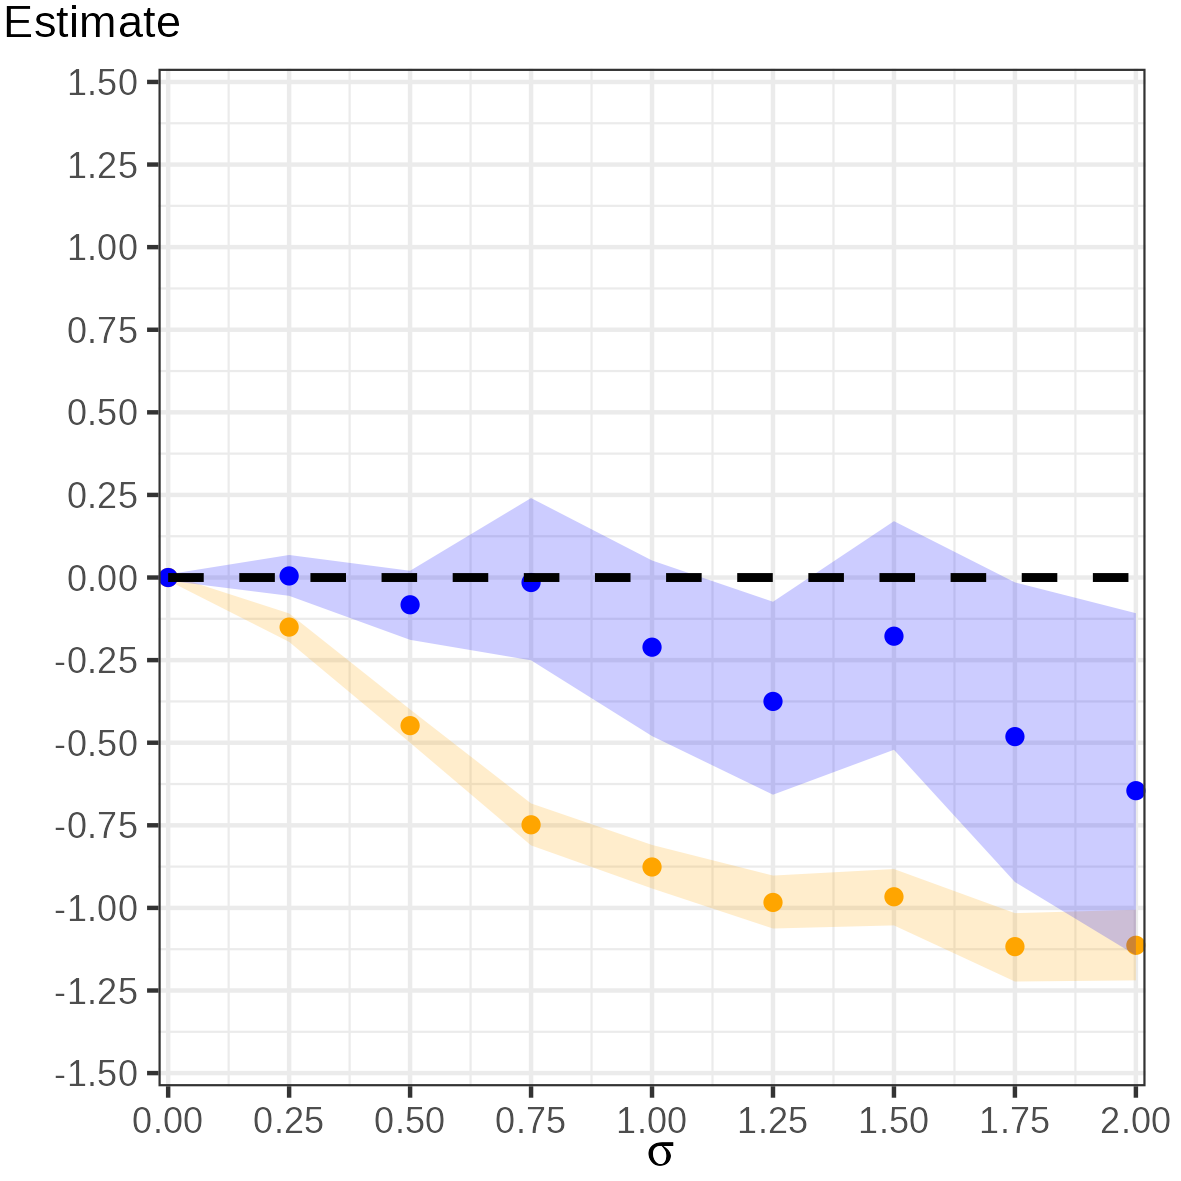
\includegraphics[width=\textwidth]{
            ../programs/simulations/sim-output/sigma-directeffect-bias.png}
    \end{subfigure}
    \begin{subfigure}[c]{0.475\textwidth}
        \centering
        \caption{$\hat{\text{AIE}} \;-$ AIE.}
        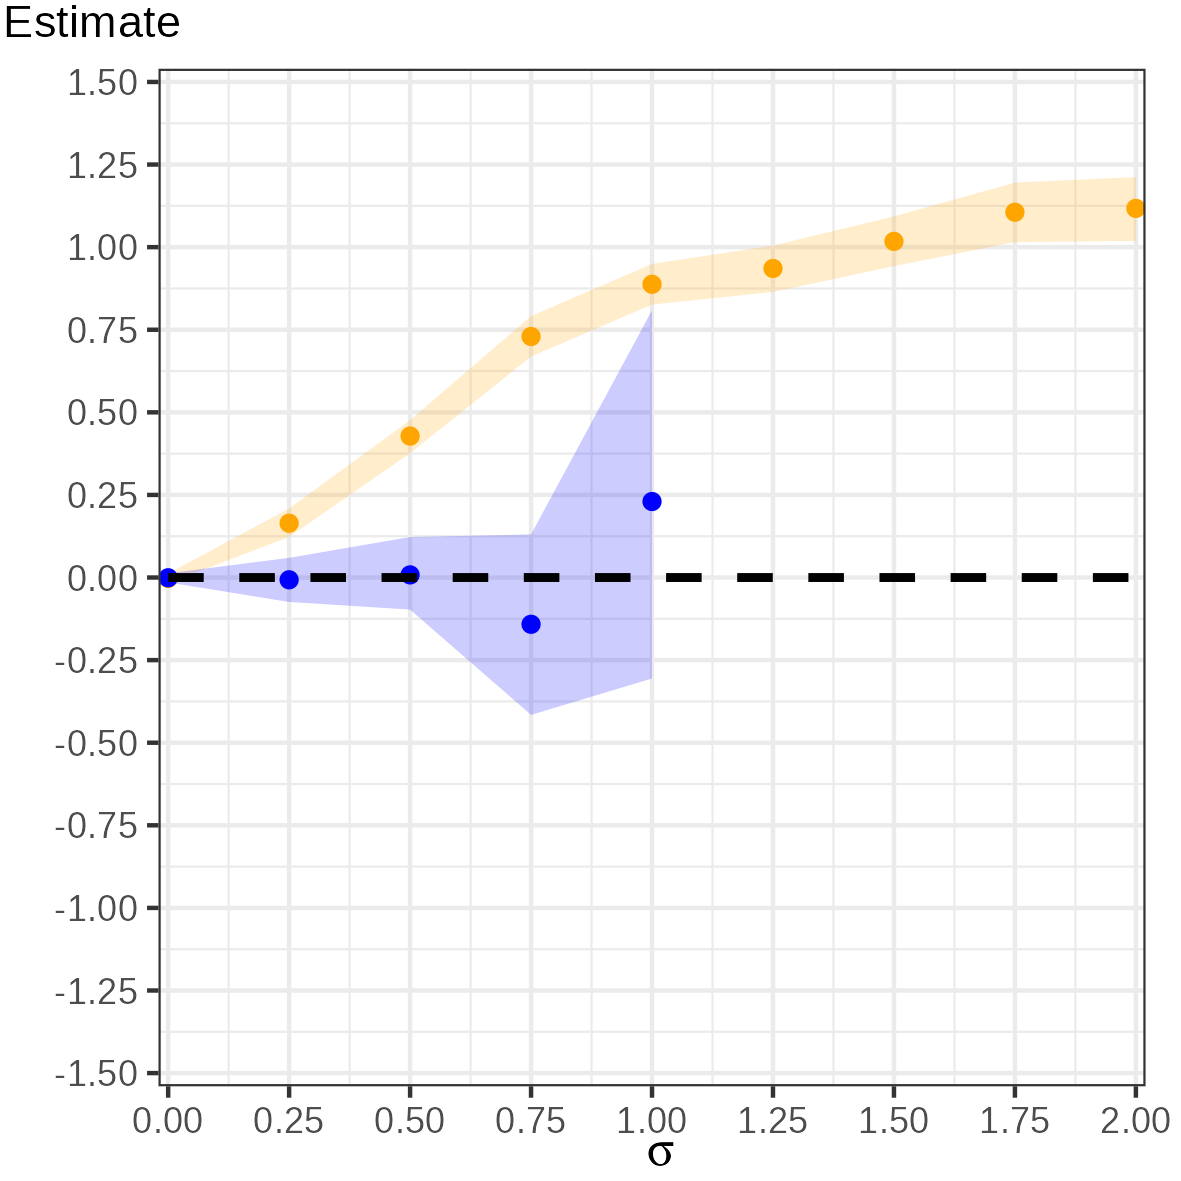
\includegraphics[width=\textwidth]{
            ../programs/simulations/sim-output/sigma-indirecteffect-bias.png}
    \end{subfigure}
    \label{fig:sigma-bias}
    \justify
    \footnotesize    
    \textbf{Note:}
    These figures show the OLS and control function point estimates of the ADE and AIE, for $N = 10,000$ sample size, minus the true value of the ADE and AIE, respectively.
    $y$-axis value of zero means the point estimate had estimated the ADE, or AIE, exactly.
    Points are points estimates from data simulated with a given $\rho = 0.5$ value, varying the $\sigma_0 = \sigma, \sigma_1 = 2\sigma$ values.
    Orange represents OLS estimates, blue the control function approach.
    Shaded regions are the 95\% confidence intervals from 1,000 bootstraps each.
\end{figure}

\begin{figure}[h!]
    \caption{OLS versus Control Function Estimates of CM Effects, varying $\sigma_1$ relative to $\sigma_0 = 1$.}
    \begin{subfigure}[c]{0.475\textwidth}
        \centering
        \caption{ADE.}
        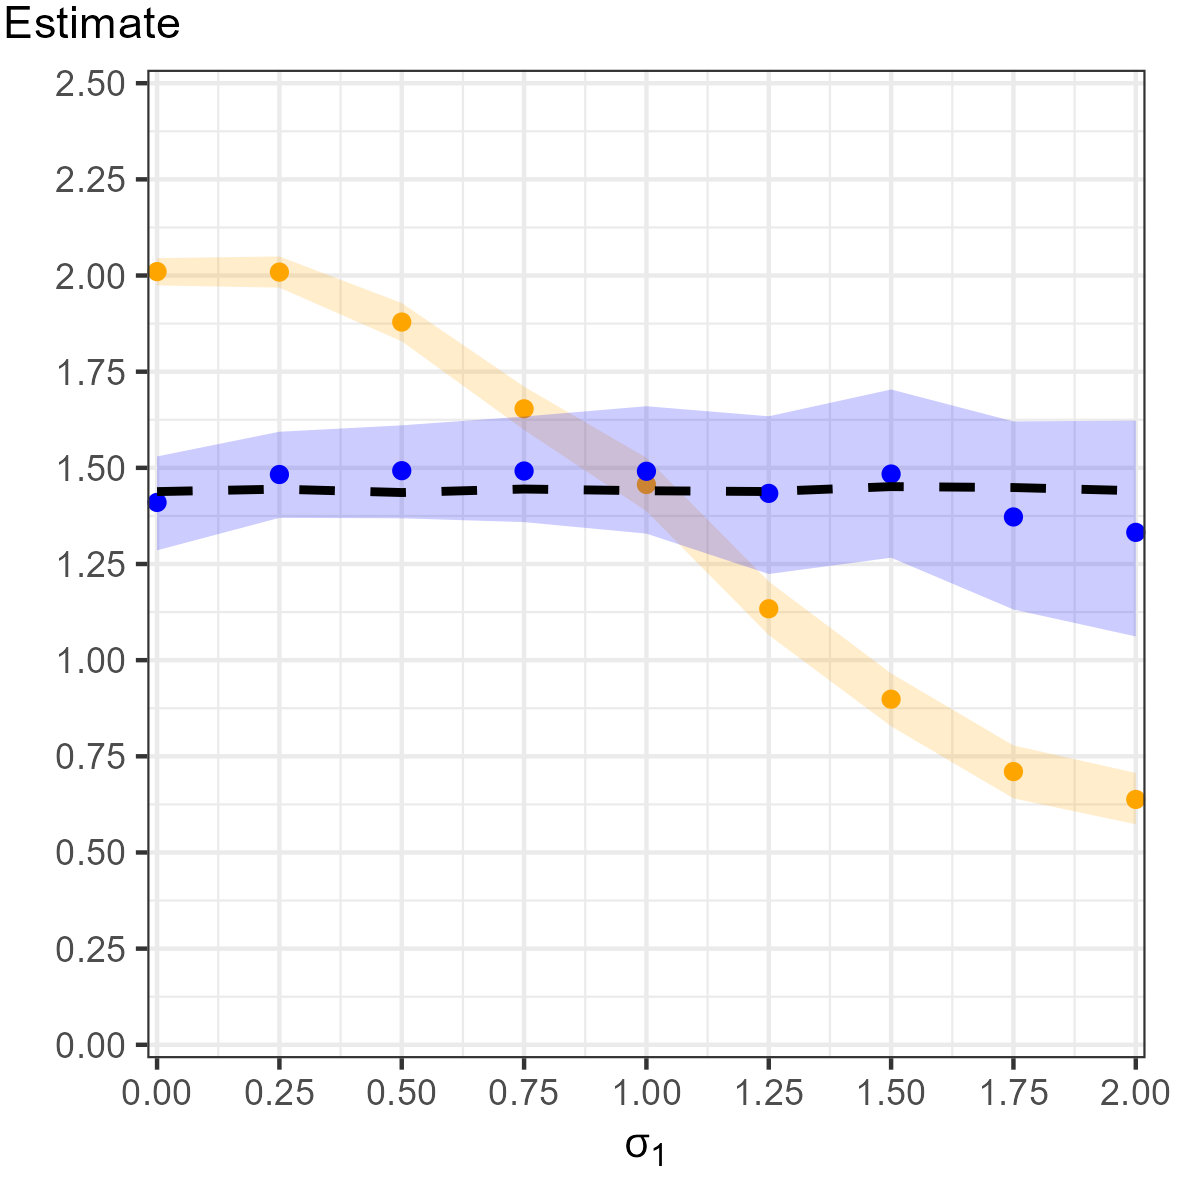
\includegraphics[width=\textwidth]{
            ../programs/simulations/sim-output/sigma-1-directeffect-bias.png}
    \end{subfigure}
    \begin{subfigure}[c]{0.475\textwidth}
        \centering
        \caption{AIE.}
        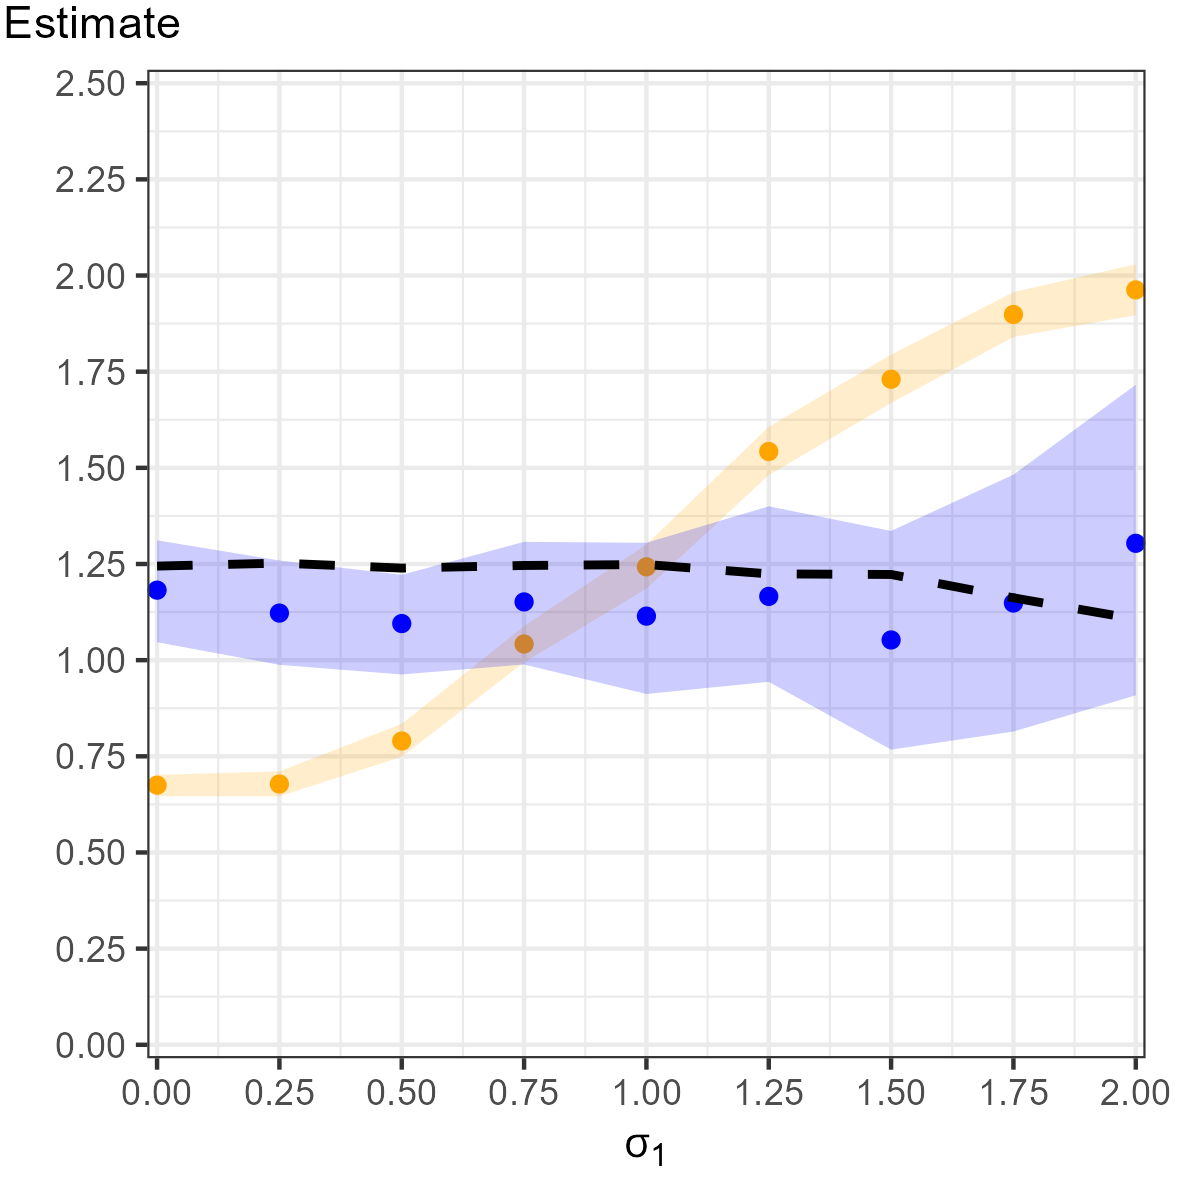
\includegraphics[width=\textwidth]{
            ../programs/simulations/sim-output/sigma-1-indirecteffect-bias.png}
    \end{subfigure}
    \label{fig:sigma-1-bias}
    \justify
    \footnotesize    
    \textbf{Note:}
    These figures show the OLS and control function estimates of the ADE and AIE, for $N = 10,000$ sample size.
    The black dashed line is the true value, points are points estimates from data simulated with a given $\rho = 0.5, \sigma_0 = 1$ and $\sigma_1$ varied across $[0, 2]$.
    Shaded regions are the 95\% confidence intervals;
    orange are the OLS estimates, blue the control function approach.
\end{figure}
